\chapter{Introduction}

When we try to research on the topic about cryptography, a fundamental question is: how can we tell whether a cryptographic construction is “really secure” against real-world attackers? In particular, there are two routes. One is to experiments to find attacks and counterexamples. The other is to provide security proofs that can be independently reproduced and proved. Our project follows the second approach: we translate a bidirectional security into executable games and reductions, and use a proof assistant to automatically check each step of the reasoning.


In particular, we study a bilateral equivalence established in~\cite{fuchsbauer2018}, between the ElGamal Key Encapsulation Mechanism (\KEM) and its security in the attack model that allows decryption queries before the challenge is issued, denoted \INDCCAone and a algebraic hardness assumption, the q-Decisional Diffie–Hellman problem (\qDDH) in the Algebraic Group Model (AGM). All the terms mentioned above is detailed explained in the Section~\ref{sec:background1}.


The central claim of our work is that, under accurate and suitable formalisation, is it possible to prove that breaking the \INDCCAone security of the ElGamal \KEM is basically the same task as distinguishing the two distributions in the \qDDH problem for the same parameters. 




\section{Motivation}
\label{sec:motivate}

In cryptographic security analysis, the \emph{computational model} provides a formal framework which defines the adversaries' capabilities and constraints of adversaries when attacking a cryptographic scheme to determine the security of a cryptosystem. 

In particular, the \emph{standard model} (explained in subsection~\ref{subsec:sm}) imposes minimal restrictions which refers to the computational framework where the adversary is assumed to be bounded only by the time and computational power, while \emph{idealized models}(explained in subsection~\ref{subsec:im}) such as the random oracle model
or generic group model impose additional constraints, where the adversaries are assumed to only accessible to a random encoding of group elements, rather than the concrete and efficiently computable representations. The Algebraic Group Model (AGM)(explained in subsection~\ref{sec:agm-background}), introduced by Fuchsbauer, Kiltz, and Loss\cite{fuchsbauer2018}, provides a middle ground between the standard model and idealized models mentioned above. The full explanation of these models lies in the section~\ref{sec:crypto-models}.

In the AGM, adversaries are restricted to be \emph{algebraic}, meaning they can only produce group elements for which they can provide explicit representations in terms of previously seen group elements. This restriction represents the intuition that adversaries cannot produce group elements arbitrarily but must construct them through the algebraic structure of existing elements.

The AGM has proven particularly valuable for analyzing the security of cryptographic schemes based on discrete logarithm assumptions. It enables proofs that would be infeasible in the standard model while avoiding the oversimplifications of purely idealized settings\cite{Bauer2021}. Recent work has highlights that many schemes, including digital signatures~\cite{fersch2018} and KEMs derived from ElGamal, can be proven secure under standard hardness assumptions when analyzed in the AGM.



Our work builds on this foundation by leveraging AGM-style techniques to indicates the IND-CCA1 security of ElGamal-based \KEM under the \qDDH assumption. 

In addition, as the main foundation of our work, Fuchsbauer, Kiltz, and Loss~\cite{fuchsbauer2018} established 
a bilateral reduction between the IND-CCA1 security of ElGamal-based KEM and 
the q-DDH assumption, providing a paper proof of this equivalence. Based 
on their theoretical framework, our work aims to provide a machine-checked 
verification of this reduction using the EasyCrypt. We want our
formalization translates their high-level cryptographic arguments into entire
mechanized proofs, making explicit all reasoning that is implicit in the 
original paper proof and ensuring correctness.

The proofs are mechanized in the EasyCrypt proof assistant\cite{easycrypt}, which is tailored for game-based cryptographic proofs at code level and gives support for common proof techniques, for instance, byequiv transformations, probabilistic reasoning, random variable transformations and algebraic manipulation techniques, it has been widely applied to build the security of the majority of cryptographic primitives and to connect with formalized proofs and their particular implementations. The detailed easycrypt introduction is in the Section~\ref{sec:easycrypt-framework}







\section{Problem Statement}
\label{sec:problemstate}

The central question we address is:

\begin{quote}
\emph{Can we introduce a formal and bidirectional methodology, to prove the equivalence between breaking IND-CCA1 security of ElGamal-based \KEM and solving the q-DDH problem, with both reductions machine-checked?}
\end{quote}

This research question requires several challenges that required to be carefully addressed in order to build a mechanized proof

\begin{enumerate}
\item \textbf{Reduction Construction}: 


The reduction from~\cite{fuchsbauer2018} provides bidirectional transformations between IND-CCA1 adversaries and q-DDH distinguishers.
The first important part of our work is to formalize both reductions using EasyCrypt. Precisely, the reduction is required to convert any IND-CCA1 adversary against ElGamal-based \KEM into a distinguisher for q-DDH, and conversely, it should also established an approach to transform a q-DDH distinguisher into IND-CCA1 adversary. This reduction embeds the q-DDH instance into the \KEM security game, relating the adversarial advantages in both problems
.

\item \textbf{Oracle Simulation}: 

An important aspect of the reduction is the decryption oracle simulator, the oracle is required to consistently answer the queries from adversaries while avoiding information leakage that would trivialize the \qDDH challenge. In our formalization, we should mechanize how the simulators handles decryption queries in a way that is consistent with the \qDDH challenge while preserving the hidden exponent. We should follow the AGM setting~\cite{cong2022}, where adversaries should provide linear representations of ciphertexts, allowing the simulator to compute the responses based on this representations. Our easycrypt formaliztion should verify this simulation correctly preserve consistency without information leakage.





\item \textbf{Formal Verification}: 

Beyond the high-level reduction, a key challenge lies in mechanizing the proof within EasyCrypt, which requires converting the theoretical reduction proof from \texttt{A.3} in ~\cite{fuchsbauer2018} into a entirely machine-checked one, it requires us to making explicit all reasoning that is left implicit in the paper proof. For instance, we need to encode all probabilistic reasoning, hybrid argument and algebraic manipulation correctly. In contrast to the traditional paper proofs where intuition often fill in the gaps, mechanized verification requires complete formal rigor for each step such as constraints on length and the randomness-preserving transformations. This part is the most significant part of our work and the main challenge is reconciling the intuitive algebraic reasoning with the strict requirements of EasyCrypt.


\item \textbf{Learning EasyCrypt}: 

An additional main challenge is mastering the EasyCrypt proof assistant itself, which requires understanding both its proof logic (pRHL) and its tactical language. At the initial stage of this project, EasyCrypt was an unfamiliar tool for me. Mastering the EasyCrypt requires extensive reading of the reference manual and sample code, repeated experimentation with different proof strategies, and continuous learning and adjustment during the ongoing formalization process.




\end{enumerate}

% \begin{figure}[htbp]
% \centering
% \begin{tikzpicture}[
%     node distance=3cm,
%     game/.style={rectangle, draw, fill=blue!15, text width=5.5cm, text centered, minimum height=3.5cm, rounded corners=4pt},
%     scheme/.style={rectangle, draw, fill=green!15, text width=4.5cm, text centered, minimum height=2.8cm, rounded corners=4pt},
%     reduction/.style={rectangle, draw, fill=orange!15, text width=4cm, text centered, minimum height=2cm, rounded corners=4pt},
%     arrow/.style={->, thick, >=stealth},
%     equiv/.style={<->, very thick, blue, >=stealth}
% ]

% % IND-CCA1 Game
% \node[game] (indcca-game) at (-10.5,5) {
%     \textbf{IND-CCA1 Game}\\[0.3cm]
%     \footnotesize
%      $(pk, sk) \leftarrow \text{Gen}()$\\
%      $b' \leftarrow A^{\text{Dec},\text{Enc}}(pk)$\\
%      Return $b'$\\[0.3cm]
%     \textbf{Dec}$(C)$ // Before Enc\\
%      $K \leftarrow \text{Dec}(C, sk)$\\
%      Return $K$\\[0.3cm]
%     \textbf{Enc}$()$ // One time\\
%      $(K_0^*, C^*) \leftarrow \text{Enc}(pk)$\\
%      $K_1^* \leftarrow \mathcal{K}$\\
%      Return $(K_b^*, C^*)$
% };

% % q-DDH Game  
% \node[game] (qddh-game) at (0.5,5) {
%     \textbf{q-DDH Game}\\[0.3cm]
%     \footnotesize
%      $x, r, z \leftarrow \mathbb{Z}_p$\\
%      $b' \leftarrow A(g^x, g^{x^2}, \ldots, g^{x^q},$\\
%     \phantom{01 $b' \leftarrow A($}$g^r, g^{xr+zb})$\\
%      Return $b'$
% };

% % ElGamal Scheme
% \node[scheme] (elgamal) at (-10.5,-8) {
%     \textbf{ElGamal KEM}\\[0.3cm]
%     \footnotesize
%     \textbf{Gen}$(\mathcal{G})$:\\
%      $x \leftarrow \mathbb{Z}_p$\\
%      $X := g^x$\\
%     Return $(pk, sk) := (X, x)$\\[0.3cm]
%     \textbf{Enc}$(pk)$:\\
%      $r \leftarrow \mathbb{Z}_p$\\
%     $C := g^r$\\
%      $K := X^r$\\
%      Return $(K, C)$\\[0.3cm]
%     \textbf{Dec}$(C, sk)$:\\
%      If $C \notin \mathcal{G}$ Return $\perp$\\
%      $K := C^x$\\
%      Return $K$
% };

% % q-DDH Problem Structure
% \node[scheme] (qddh-structure) at (0.5,-6) {
%     \textbf{q-DDH Structure}\\[0.3cm]
%     \footnotesize
%     Given: $(g^x, g^{x^2}, \ldots, g^{x^q}, g^r, T)$\\[0.3cm]
%     Distinguish:\\
%     • $T = g^{xr}$ (real)\\
%     • $T = g^{xr+z}$ (random)\\[0.3cm]
%     where $x, r, z \leftarrow \mathbb{Z}_p$
% };
% % Forward Reduction
% \node[reduction] (forward-red) at (-7.5,-0.5) {
%     \textbf{${\text{A\_from\_INDCCA1}}(B)$}\\[0.2cm]
%     \footnotesize
%     • Receives q-DDH challenge\\
%     • Sets $pk = g^x$\\
%     • Simulates limited Dec oracle\\
%     • Uses linear representations\\
%     • Outputs q-DDH decision
% };

% % Backward Reduction
% \node[reduction] (backward-red) at (-2.5,0.5) {
%     \textbf{${\text{B\_from\_qDDH}}(A)$}\\[0.2cm]
%     \footnotesize
%     • Embeds q-DDH challenge\\
%     • Simulates IND-CCA1 game\\
%     • Programs challenge ciphertext\\
%     • Uses same oracle discipline\\
%     • Outputs IND-CCA1 guess
% };
% % Main equivalence
% \draw[equiv] (indcca-game) -- (qddh-game) node[midway, above] {\textbf{Tight Bilateral Equivalence}};

% % Connections to schemes
% \draw[arrow] (indcca-game) -- (elgamal) node[midway, left] {uses};
% \draw[arrow] (qddh-game) -- (qddh-structure) node[midway, right] {based on};

% % Reduction arrows
% \draw[arrow] (elgamal) -- (forward-red) node[midway, below left, sloped] {input};
% \draw[arrow] (forward-red) -- (qddh-structure) node[midway, below right, sloped] {output};

% \draw[arrow] (qddh-structure) -- (backward-red) node[midway, below right, sloped] {input};
% \draw[arrow] (backward-red) -- (elgamal) node[midway, below left, sloped] {output};

% % Oracle simulation details
% \node[draw, fill=yellow!10, text width=8cm, rounded corners] (oracle-details) at (-3.75,-10) {
%     \textbf{Key Technical Components:}\\[0.2cm]
%     • Limited Decryption Oracle: requires $c = \text{prodEx}(l, z)$\\
%     • Linear Algebra Library: \texttt{prodEx}, \texttt{addv}, \texttt{scalev}, \texttt{sumv}\\
%     • 30+ Supporting Lemmas: distributivity, scaling, base reduction\\
%     • Tight Analysis: $\mathsf{Adv}_{\text{IND-CCA1}} = \mathsf{Adv}_{\text{q-DDH}}$
% };

% \draw[arrow, dotted] (forward-red) -- (oracle-details);
% \draw[arrow, dotted] (backward-red) -- (oracle-details);

% \end{tikzpicture}
% \caption{Detailed bilateral reduction between IND-CCA1 security of ElGamal-based \KEM and \qDDH hardness, showing the complete game structures and algorithmic details.}
% \label{fig:detailed-bilateral-reduction}
% \end{figure}



\section{Main Contributions}

This thesis provides an entire machine-checked formalization of the bidirectional reduction between \INDCCAone security of ElGamal \KEM and \qDDH from ~\cite{fuchsbauer2018}. The mechanization process handles the key challenges in formal verification and indicates the feasibility of machine checking the AGM based cryptographic proofs. The main contributions are:



\begin{enumerate}




\item \textbf{Complete Bilateral Reduction Formalization}: 

We provide a machine-checked formalization in EasyCrypt of both directions of the reduction from ~\cite{fuchsbauer2018}, to be more specific, we try to construct the computational equivalence by the following code format:

We formalize the \texttt{qDDH\_Implies\_INDCCA1\_ElGamal }and \newline \texttt{INDCCA1\_ElGamal\_Implies\_qDDH} lemma, verifying the equivalence between q-DDH hardness and IND-CCA1 security from ~\cite{fuchsbauer2018}:
\begin{equation}
\label{eq:bilateral-equivalence}
\Pr[\text{IND\_CCA1\_P}(\text{ElGamal}, B).\text{main}() : \text{res}] = 
\Pr[\text{QDDH}(A_{\text{from\_INDCCA1}}(B)).\text{main}() : \text{res}]
\end{equation}

The formalization we construct verify the correctness of the relationship claimed in the original paper~\cite{fuchsbauer2018}

\item \textbf{Oracle Simulation Technique}: 

We formalized the decryption oracle simulation technique from~\cite{fuchsbauer2018} using EasyCrypt, which leverages algebraic representations to answer the adversaries' queries. In doing so, we  handle the challenge in encoding the extraction of representation while ensuring the simulator preserving the consistency invariants.

\item \textbf{Linear Algebra Manipulation framework}: 

To make the formalization more efficient, we develop a framework consists of a collection of EasyCrypt operators and corresponding lemmas that able to solve linear algebraic operations over exponents:
  \begin{itemize}
  \item Core operators: \texttt{prodEx}, \texttt{addv}, \texttt{scalev}, \texttt{sumv}, \texttt{shift\_trunc}
  \item Over 30  lemmas of distributivity, scaling, base reduction, and vector operations
  \item Reusable components for AGM proofs with linear combinations
  \end{itemize}

\item \textbf{Complete Machine-checked proof}: 

The entire proof of theorem is mechanized using the EasyCrypt, consists of over 2000 lines of code, including lemmas, defintions and proof scripts. Our work shows that sophisticated AGM-based reductions and oracle simulations and proof process can be successfully translated into code format.


\item \textbf{Insights from Formalization}: 

Through the entire process of formalization, I obtained detailed understanding of the reduction's structure and the challenges of formalizing AGM-based proofs. In addition, I think it will be more easy for me to using EasyCrypt to do future formalizing, which may be valuable for future efforts to mechanize similar cryptographic proofs.

\end{enumerate}





\section{Technical Overview}

Figure~\ref{fig:detailed-bilateral-reduction} indicates an overview of the reduction framework from~\cite{fuchsbauer2018} that we formalize in EasyCrypt.

At a high level, our goal is to using EasyCrypt to show that the capability to break the IND-CCA1 security of the ElGamal-based \KEM\ is computationally equivalent to handling the \qDDH\ problem. Our formalization mechanizes both directions of this equivalence, verifying that adversaries can be transformed in either direction while preserving their computational advantages.

In the \textbf{first direction},the reduction converts any adversary of ElGamal \KEM\ under chosen-ciphertext attacks into an algorithm that handle the \qDDH\ challenge. 
In the \textbf{reverse direction}, the reduction transforms an \INDCCAone adversary from any \qDDH distinguisher by embedding the \KEM challenge into a \qDDH challenge.

A key technical point is the leverage of \textbf{algebraic tracking}, inspired by the Algebraic Group Model~\cite{fuchsbauer2018}. Where every group element generated during the simulation is represented as a linear combination of previously known ones, ensures that simulated oracles answer consistently and guarantees every adversarial action has a verifiable algebraic explanation.

Finally, the entire framework, containing oracle simulations, linear algebra operators (\texttt{prodEx}, \texttt{addv}, \texttt{scalev}, \texttt{sumv}) and supporting lemmas is implemented and mechanically verified in the \textsc{EasyCrypt} proof assistant, which guarantees the correspondence between the two games is not only theoretically sound but also \emph{machine-checked}.

By completing all the preparation work we mentioned above, making our machined-checked proof stage become efficiency and easy to prove the equivalence we mentioned: equation~\ref{eq:bilateral-equivalence}

\newpage



\begin{figure}[H]
\centering
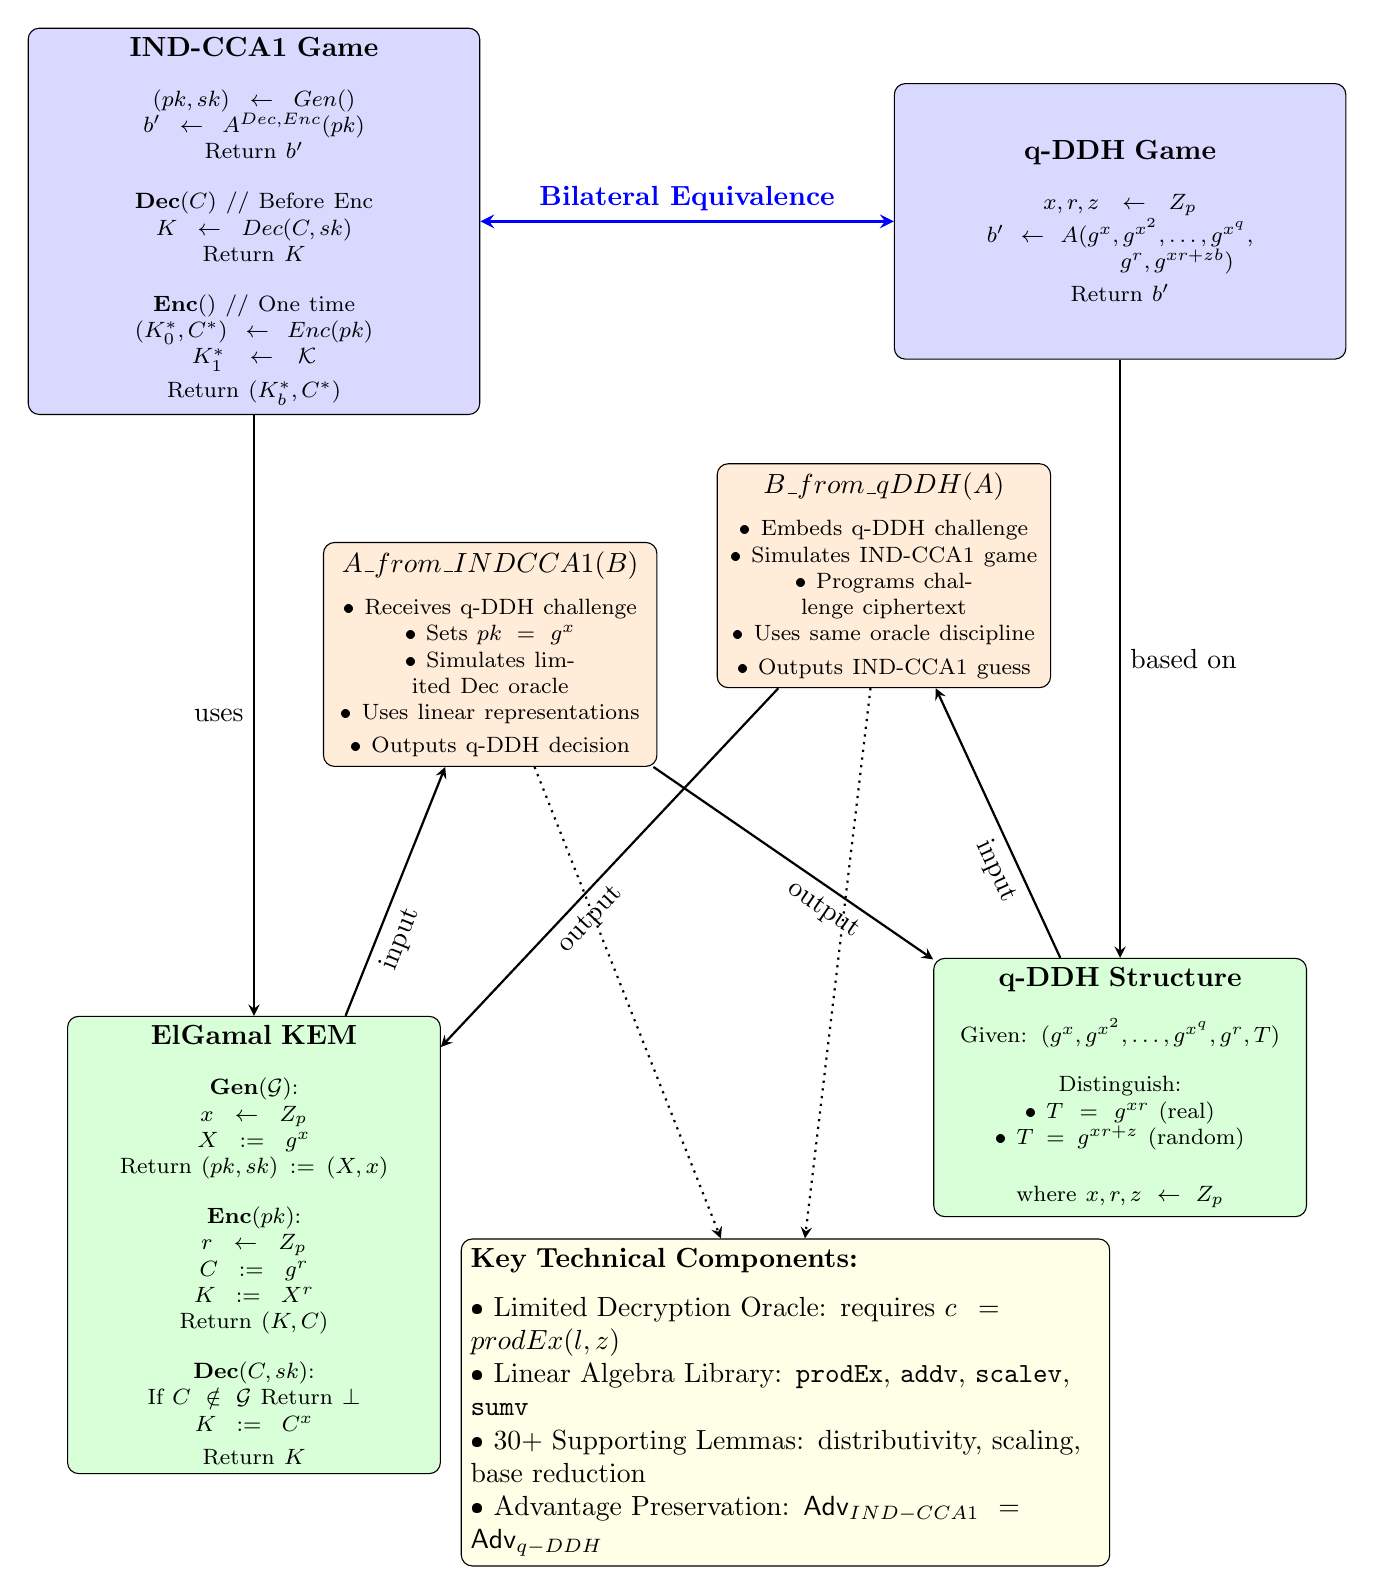
\begin{tikzpicture}[
    node distance=3cm,
    game/.style={rectangle, draw, fill=blue!15, text width=5.5cm, text centered, minimum height=3.5cm, rounded corners=4pt},
    scheme/.style={rectangle, draw, fill=green!15, text width=4.5cm, text centered, minimum height=2.8cm, rounded corners=4pt},
    reduction/.style={rectangle, draw, fill=orange!15, text width=4cm, text centered, minimum height=2cm, rounded corners=4pt},
    arrow/.style={->, thick, >=stealth},
    equiv/.style={<->, very thick, blue, >=stealth}
]

% IND-CCA1 Game
\node[game] (indcca-game) at (-10.5,5) {
    \textbf{IND-CCA1 Game}\\[0.3cm]
    \footnotesize
     $(pk, sk) \leftarrow \text{Gen}()$\\
     $b' \leftarrow A^{\text{Dec},\text{Enc}}(pk)$\\
     Return $b'$\\[0.3cm]
    \textbf{Dec}$(C)$ // Before Enc\\
     $K \leftarrow \text{Dec}(C, sk)$\\
     Return $K$\\[0.3cm]
    \textbf{Enc}$()$ // One time\\
     $(K_0^*, C^*) \leftarrow \text{Enc}(pk)$\\
     $K_1^* \leftarrow \mathcal{K}$\\
     Return $(K_b^*, C^*)$
};

% q-DDH Game  
\node[game] (qddh-game) at (0.5,5) {
    \textbf{q-DDH Game}\\[0.3cm]
    \footnotesize
     $x, r, z \leftarrow \mathbb{Z}_p$\\
     $b' \leftarrow A(g^x, g^{x^2}, \ldots, g^{x^q},$\\
    \phantom{01 $b' \leftarrow A($}$g^r, g^{xr+zb})$\\
     Return $b'$
};

% ElGamal Scheme
\node[scheme] (elgamal) at (-10.5,-8) {
    \textbf{ElGamal KEM}\\[0.3cm]
    \footnotesize
    \textbf{Gen}$(\mathcal{G})$:\\
     $x \leftarrow \mathbb{Z}_p$\\
     $X := g^x$\\
    Return $(pk, sk) := (X, x)$\\[0.3cm]
    \textbf{Enc}$(pk)$:\\
     $r \leftarrow \mathbb{Z}_p$\\
    $C := g^r$\\
     $K := X^r$\\
     Return $(K, C)$\\[0.3cm]
    \textbf{Dec}$(C, sk)$:\\
     If $C \notin \mathcal{G}$ Return $\perp$\\
     $K := C^x$\\
     Return $K$
};

% q-DDH Problem Structure
\node[scheme] (qddh-structure) at (0.5,-6) {
    \textbf{q-DDH Structure}\\[0.3cm]
    \footnotesize
    Given: $(g^x, g^{x^2}, \ldots, g^{x^q}, g^r, T)$\\[0.3cm]
    Distinguish:\\
    • $T = g^{xr}$ (real)\\
    • $T = g^{xr+z}$ (random)\\[0.3cm]
    where $x, r, z \leftarrow \mathbb{Z}_p$
};
% Forward Reduction
\node[reduction] (forward-red) at (-7.5,-0.5) {
    \textbf{${\text{A\_from\_INDCCA1}}(B)$}\\[0.2cm]
    \footnotesize
    • Receives q-DDH challenge\\
    • Sets $pk = g^x$\\
    • Simulates limited Dec oracle\\
    • Uses linear representations\\
    • Outputs q-DDH decision
};

% Backward Reduction
\node[reduction] (backward-red) at (-2.5,0.5) {
    \textbf{${\text{B\_from\_qDDH}}(A)$}\\[0.2cm]
    \footnotesize
    • Embeds q-DDH challenge\\
    • Simulates IND-CCA1 game\\
    • Programs challenge ciphertext\\
    • Uses same oracle discipline\\
    • Outputs IND-CCA1 guess
};
% Main equivalence
\draw[equiv] (indcca-game) -- (qddh-game) node[midway, above] {\textbf{Bilateral Equivalence}};

% Connections to schemes
\draw[arrow] (indcca-game) -- (elgamal) node[midway, left] {uses};
\draw[arrow] (qddh-game) -- (qddh-structure) node[midway, right] {based on};

% Reduction arrows
\draw[arrow] (elgamal) -- (forward-red) node[midway, below left, sloped] {input};
\draw[arrow] (forward-red) -- (qddh-structure) node[midway, below right, sloped] {output};

\draw[arrow] (qddh-structure) -- (backward-red) node[midway, below right, sloped] {input};
\draw[arrow] (backward-red) -- (elgamal) node[midway, below left, sloped] {output};

% Oracle simulation details
\node[draw, fill=yellow!10, text width=8cm, rounded corners] (oracle-details) at (-3.75,-10) {
    \textbf{Key Technical Components:}\\[0.2cm]
    • Limited Decryption Oracle: requires $c = \text{prodEx}(l, z)$\\
    • Linear Algebra Library: \texttt{prodEx}, \texttt{addv}, \texttt{scalev}, \texttt{sumv}\\
    • 30+ Supporting Lemmas: distributivity, scaling, base reduction\\
    • Advantage Preservation: $\mathsf{Adv}_{\text{IND-CCA1}} = \mathsf{Adv}_{\text{q-DDH}}$
};

\draw[arrow, dotted] (forward-red) -- (oracle-details);
\draw[arrow, dotted] (backward-red) -- (oracle-details);

\end{tikzpicture}
\caption{Detailed bilateral reduction between IND-CCA1 security of ElGamal-based \KEM and \qDDH hardness, showing the complete game structures and algorithmic details.}
\label{fig:detailed-bilateral-reduction}
\end{figure}






% \subsection{Problem Structure and Games}

% The foundation of proof lies in the characterization of two computation problems:

% \subsubsection{IND-CCA1 Security Game.} 

% The indistinguishability under chosen-ciphertext attacks (IND-CCA1) security game for ElGamal \KEM proceeds as follows: The challenger first introduce a key pair $\text{Gen}()\rightarrow(pk,sk)$ where $pk = g^x$ and $sk = x$ for a randomly chosen $x \leftarrow \mathbb{Z}_p$. Then, the adversary $A$ is given the public key $pk$ and then make decryption queries to a oracle $\text{Dec}(C, sk)$ that returns $K = C^x$ for valid ciphertexts $C \in \mathcal{G}$. At some point, the adversary requests a challenge by calling the encryption oracle only once. The challenger computes $ \text{Enc}(pk)\rightarrow(K_0^*, C^*)$ where $C^* = g^r$ and $K_0^* = (g^x)^r = g^{xr}$ for a  random $ \mathbb{Z}_p \rightarrow r$, then selects a random key $ \mathcal{K} \rightarrow K_1^*$, and finally return $(K_b^*, C^*)$ for a random bit $b$. Finally, The adversary will outputs a guess $b'$ and wins if $b' = b$.

% The algorithm specification\cite{fuchsbauer2018} is detailed in Figure~\ref{fig:indcca1-algorithm}.

% \begin{figure}[H]
% \centering
% \footnotesize
% \begin{tabular}{|p{15cm}|}
% \hline
% \multicolumn{1}{|c|}{\textbf{IND-CCA1$_{\text{EG},\mathcal{G}}^A$ Security Game for ElGamal}} \\
% \hline
% \textbf{Algorithm:} \\
% 00 $x \leftarrow \mathbb{Z}_p$ \\
% 01 $X := g^x$ \\
% 02 $b' \leftarrow A^{\text{Dec},\text{Enc}}(X)$ \\
% 03 Return $b'$ \\
% \hline
% \textbf{Oracles Available to Adversary } $A$\textbf{:} \\
% $\bullet$ \textbf{Dec}$(C)_a$ // Before Enc is called \\
% \phantom{$\bullet$} 04 If $C \notin \mathcal{G}$ Return $\perp$ \\
% \phantom{$\bullet$} 05 $K := C^x$ \\
% \phantom{$\bullet$} 06 Return $K$ \\
% \\
% $\bullet$ \textbf{Enc}$()$ // One time only \\
% \phantom{$\bullet$} 07 $r \leftarrow \mathbb{Z}_p$ \\
% \phantom{$\bullet$} 08 $C^* := g^r$ \\
% \phantom{$\bullet$} 09 $K^* := X^r$ \\
% \phantom{$\bullet$} 10 $K_1^* \leftarrow \mathcal{K}$ // random key \\
% \phantom{$\bullet$} 11 $b \leftarrow \{0,1\}$ \\
% \phantom{$\bullet$} 12 Return $(K_b^*, C^*)$ \\
% \hline
% \textbf{ElGamal KEM Operations:} \\
% $\bullet$ \textbf{Gen}$(\mathcal{G}) \rightarrow (pk, sk)$: $x \leftarrow \mathbb{Z}_p$; $X := g^x$; Return $(X, x)$ \\
% $\bullet$ \textbf{Enc}$(pk) \rightarrow (K, C)$: $r \leftarrow \mathbb{Z}_p$; $C := g^r$; $K := pk^r$; Return $(K, C)$ \\
% $\bullet$ \textbf{Dec}$(C, sk) \rightarrow K$: If $C \notin \mathcal{G}$ Return $\perp$; $K := C^{sk}$; Return $K$ \\
% \hline
% \textbf{Advantage Definition:} \\
% $\mathsf{Adv}^{\text{IND-CCA1}}_{\text{ElGamal}}(A) = \left|\Pr[b' = b] - \frac{1}{2}\right|$ \\
% where $b$ is the random bit used in the Enc oracle \\
% \hline
% \textbf{Security Goal:} \\
% Adversary $A$ should not be able to distinguish between $K_0^* = g^{xr}$ (real key) and $K_1^*$ (random key) \\
% even with access to decryption oracle before receiving the challenge $(K_b^*, C^*)$ \\
% \hline
% \end{tabular}
% \caption{IND-CCA1 security game for ElGamal encryption. The adversary has access to a decryption oracle before the challenge phase, then must distinguish between a real session key and a random key.}
% \label{fig:indcca1-algorithm}
% \end{figure}






% \subsubsection{q-DDH Problem.} The q-Decisional Diffie-Hellman (q-DDH) problem will ask one to distinguish between two distributions over group elements. 
% By given a tuple $(g^x, g^{x^2}, \ldots, g^{x^q}, g^r, T)$ where $x, r \leftarrow \mathbb{Z}_p$ are random, the attacker must determine whether $T = g^{xr}$ (real distribution) or $T = g^{xr+z}$ for a random $z \leftarrow \mathbb{Z}_p$ (random distribution).

% The specification\cite{fuchsbauer2018} is detailed below in Figure~\ref{fig:qddh-algorithm}.


% \begin{figure}[H]
% \centering
% \footnotesize
% \begin{tabular}{|p{15cm}|}
% \hline
% \multicolumn{1}{|c|}{\textbf{q-DDH$_{\mathcal{G},q}^A$ Problem}} \\
% \hline
% \textbf{Algorithm:} \\
% 00 $x, r, z \leftarrow \mathbb{Z}_p$ \\
% 01 $b \leftarrow \{0,1\}$ \\
% 02 $T_0 := g^{xr}$, $T_1 := g^{xr+z}$ \\
% 03 $b' \leftarrow A(g^x, g^{x^2}, \ldots, g^{x^q}, g^r, T_b)$ \\
% 04 Return $b'$ \\
% \hline
% \textbf{Challenge Structure Given to Distinguisher } $A$\textbf{:} \\
% $\bullet$ \textbf{Powers of } $x$: $(g^x, g^{x^2}, g^{x^3}, \ldots, g^{x^q})$ \\
% $\bullet$ \textbf{Random element:} $g^r$ where $r \leftarrow \mathbb{Z}_p$ \\
% $\bullet$ \textbf{Target element:} $T \in \{g^{xr}, g^{xr+z}\}$ where $z \leftarrow \mathbb{Z}_p$ \\
% \hline
% \textbf{Distinguishing Goal:} \\
% $\bullet$ \textbf{Real distribution } $\mathcal{D}_0$: $T = g^{xr}$ (DDH tuple) \\
% $\bullet$ \textbf{Random distribution } $\mathcal{D}_1$: $T = g^{xr+z}$ (random element) \\
% \\
% Distinguisher $A$ must output a bit $b'$ indicating which distribution the challenge comes from \\
% \hline
% \textbf{Advantage Definition:} \\
% $\mathsf{Adv}^{q\text{-DDH}}_{\mathcal{G}}(A) = \left|\Pr[A(\mathcal{D}_0) = 1] - \Pr[A(\mathcal{D}_1) = 1]\right|$ \\
% where $\mathcal{D}_0 = (g^x, g^{x^2}, \ldots, g^{x^q}, g^r, g^{xr})$ \\
% and $\mathcal{D}_1 = (g^x, g^{x^2}, \ldots, g^{x^q}, g^r, g^{xr+z})$ \\
% \hline
% \textbf{Hardness Assumption:} \\
% For any probabilistic polynomial-time algorithm $A$: \\
% $\mathsf{Adv}^{q\text{-DDH}}_{\mathcal{G}}(A) \leq \text{negl}(\lambda)$ \\
% \\
% The q-DDH assumption states that even given the first $q$ powers of $x$, \\
% it remains computationally hard to distinguish $g^{xr}$ from $g^{xr+z}$ \\
% \hline
% \textbf{Relationship to Standard DDH:} \\
% $\bullet$ Standard DDH: Given $(g^a, g^b, g^c)$, distinguish $c = ab$ from random $c$ \\
% $\bullet$ q-DDH: Given $(g^x, \ldots, g^{x^q}, g^r, T)$, distinguish $T = g^{xr}$ from $T = g^{xr+z}$ \\
% $\bullet$ q-DDH $\Rightarrow$ DDH but the converse may not hold \\
% \hline
% \end{tabular}
% \caption{q-DDH (q-Decisional Diffie-Hellman) problem. The distinguisher receives the first $q$ powers of a secret exponent $x$ along with $g^r$ and must distinguish between $g^{xr}$ and $g^{xr+z}$ for random $z$.}
% \label{fig:qddh-algorithm}
% \end{figure}
















% \subsection{Bilateral Reduction Strategy}

% Our core technical contribution is the establishment of two reductions that bridge computational equivalence between:

% \subsubsection{Forward Reduction: ${\text{A\_from\_INDCCA1}}$.} This reduction will convert all IND-CCA1 adversary $B$ against ElGamal into a q-DDH distinguisher.,which works as follows:
% \begin{enumerate}
% \item \textbf{Challenge Reception:} It will first receiving a q-DDH challenge $(g^x, g^{x^2}, \ldots, g^{x^q}, g^r, T)$, then set the public key as $pk = g^x$.
% \item \textbf{Oracle Simulation:} Then it will leverage a limited decryption oracle that only processes queries $(C, z)$ where  adversary provides an explicit linear representation $z$ such that $C = \text{prodEx}(l, z)$, while $l = [g, g^x, \text{previous\_results}]$ is the list of group elements already known.
% \item \textbf{Challenge Programming:} Finally the adversary is expected to request the encryption challenge, that sets $C^* = g^r$ and $K^* = T$, giving the q-DDH challenge directly into the IND-CCA1 game.
% \item \textbf{Decision Extraction:} The reduction outputs the adversary's guess as its q-DDH decision.
% \end{enumerate}

% \subsubsection{Backward Reduction: ${\text{B\_from\_qDDH}}$.} This reduction converts any q-DDH distinguisher $A$ into an IND-CCA1 adversary:
% \begin{enumerate}
% \item \textbf{Challenge Embedding:} The reduction embeds the received IND-CCA1 challenge into a q-DDH problem by generating the tuple $(g^x, g^{x^2}, \ldots, g^{x^q}, C^*, K^*)$ where $x$ is the secret key and $(K^*, C^*)$ is the challenge key-ciphertext pair.
% \item \textbf{Game Simulation:} Then it will simulates the q-DDH game for the attacker by the same oracle discipline as the forward reduction.
% \item \textbf{Advantage Preservation:} The distinguisher's decision is directly translated into an IND-CCA1 guess.
% \end{enumerate}






















